\documentclass[capstone_report.tex]{subfiles}
\begin{document}
\chapter{Literature review}
This chapter presents a summary of the major contributions made to autonomous indoor flight of UAVs. We first discuss literature in relation to complete systems. Complete systems are those which have combined the control, localization, mapping and navigation sub-systems required to achieve autonomous indoor flight. We then discuss research undertaken into each of these sub-systems, insofar as they relate to autonomous flight of UAVs.\\

\section{Complete systems}
The challenges which a complete indoor autonomous UAV system needs to solve are numerous. The two fundamental differences between outdoor UAV systems and indoor systems are the lack of access to GPS data, and the presence of significantly more obstacles which need to be avoided. This leads to tighter tolerances on controller accuracy. Many approaches have been proposed and tested to resolve these issues.\\

A pivotal systems-level contribution towards a complete indoor autonomous UAV was in \cite{feicui}. The authors combined two-stage approach where the UAV would explore its environment using a laser scanner to avoid obstacles, and optical flow for basic position estimation. After the first flight, collected laser scan data was converted into a map offline using the FastSLAM algorithm, allowing future flights to be guided by the constructed map. \\

A disadvantage of post-flight mapping is the inability to map in real-time. Real-time mapping and localization is limited by the processing power onboard a UAV. A solution employed by \cite{yu:ccdc:2017} was to use a base-station computer connected to a fixed set of cameras. Data from the cameras were used to estimate the position of the UAV, and this estimate was sent via WiFi to the controller onboard the aircraft. \\

Alternatively, \cite{qzeng} attempts to make localization and mapping tractable onboard the UAV by replacing a laser scanner with a laser source which is detected by a monocular camera. A model is proposed which can track points of interest over time, matching scans at a significantly faster rate than the FastSLAM algorithm. Since this method identifies points of interest only, its utility in constructing a full map is limited.\\

More recent work has built on previous contributions with specific applications, and employing newer technologies. The system in \cite{kumar} uses two orthogonal laser scanners, and simple point-to-point scan matching method for navigation. This allows computation on newer embedded computers, removing the need for a base station. The authors also tested the UAV for pipe classification in a plant engineering/maintenance setting, with promising results.\\

The majority of successful systems in the literature use either laser scanners or laser detection as sensors. However, in \cite{mustafah} the authors employed stereo vision for positioning a UAV indoors. As a feature-based method, this approach lacks the ability to construct meaningful maps - however very acccurate position holds were able to be achieved by the authors.\\

Specifically in the field of emergency systems, Researchers at Carnegie Mellon \cite{sensorfly} successfully used a network of miniature, low cost drones collecting temperature, gas, pressure and ceiling height data to predict the propagation of a fire indoors. Low cost was a necessary design constraint as it allowed multiple drones to be deployed simultaneously to give good spatial and temporal coverage of an area. Given this limitation the ability to accurately estimate the position of the aerial vehicles was restricted as this capability is typically provided by a more expensive laser scanner unit. To rely on cheaper estimation sensors such as an inertial measurement unit (IMU) and range sensors, drones explored their environment by conducting a random walk until within a specified distance of the next drone. Interpolation was then conducted using inter-drone distance to build the 3D model.\\

An alternative solution to indoor monitoring of fire has been proposed in \cite{myeong} which developed a drone capable of mounting walls.  The ability to mount walls allows for a larger drone platform capable of carrying heavier laser scanning modules (accurate position estimation) but also the flexibility of passing through doorways vertically.  The team also showed their drone was capable of withstanding temperatures of up to 1000$^\circ C$ for 60 seconds.  It was able to achieve this by wrapping the vehicle in aramid fibre (commonly used in fire-fighters) clothing, insulating electric components with an air buffer and utilizing a thermoelectric cooler (TEC).  These promising results show that producing a drone capable of withstanding the harsh conditions is an achievable goal.\\

\section{Estimation algorithms}
In addition to having application in indoor flight systems, algorithms which jointly optimise over both a position and map configuration have a wide variety of additional applications. For this reason, the literature relating to Simultaneous Localization and Mapping (SLAM) algorithms includes many non-UAV applications. The motivation behind using such an algorithm is explained in the following chapter. This section discusses some of the variants for solving the SLAM problem in the literature.\\

While we did not write code to implement a SLAM algorithm for this project, the open source SLAM algorithm we eventually chose for URSA (Cartographer \cite{cart}) has hundreds of parameters available for configuration. The following details on SLAM algorithms is provided due to its utility in both understanding the technology options available and in configuring this component.

\subsection{Filter based SLAM}
The first detailed outline of the SLAM problem was \cite{smithcheese}. In this work, the authors used a filtering based approach with a state vector representing the current robot position, along with the position of a number of `landmarks'. A linear observation was approximated, allowing a Kalman Filter to be employed to recursively estimate the state.\\

The extraction of landmarks will depend on the sensors used. For example, if a monocular vision sensor is used, landmarks may be extracted using a Harris corner/edge detector\footnote{A Harris detector works by calculating the sum of the squared difference between each pixel in an image and its surrounding pixels. The result of this sum-of-squared difference (obtained by approximation) is then analyzed for spatial derivatives in $x$ and $y$ directions. High derivatives in both directions indicate an image corner; high derivatives in a single direction indicate an image edge. See \cite{harris}}. If a depth camera is employed, features may instead relate to the 3D structure of the enviroment measured. The most important aspect of landmarks is that they can be correlated between samples, and recognised as unique if they are revisited in the future.

There have been a number of improvements in filter based approaches over the years. More complex non-linear observation models have led to filters which are required to linearize around operating points, leading to the application of extended Kalman filters (EKF). A guide on the implementation of EKF based SLAM, including a detailed treatment of models and states used, and relevant diagrams, can be found at \cite{ekftutorial}.\\ 

EKF based appraoches typically introduce signficant linearisation errors, which have led to some researchers employing Unscented Kalman Filters to solve the problem \cite{julier}. Others have attempted to change the state parameterisation of landmark coordinates in order to make them more tractable to linearisation in the EKF \cite{julier}.\\

However, despite advances in filter based SLAM, it still suffers from significant cumulative linearisation errors when applied to models which correctly model the nonlinearities of feature observations or robot motion. Additionally, as more observations are made, more landmarks need to be added to the state vector. This requires a re-initialisation of the covariance matrix, and also causes the size of the matrix operations to grow as the algorithm continues to run. Eventually, this will exhaust computational resources. To circumvent these issues, modern filter-based SLAM algorithms impose limits on the landmarks which can be identified.\\

Another common strategy is to use sub-mapping for landmarks which are a long way from the current location or which have not been observed for a long time. This approach essentially `archives' the states associated with these landmarks by removing them from the state vector and placing their estimates in memory. This reduces the size of the state vector and therefore the complexity of the filtering operations. A full discussion on submapping approaches can be found at \cite{slamoverview}.

\subsection{Graph based SLAM}
A recent alternative to filter based SLAM requires first re-imagining the SLAM problem as a factor graph. To explain this approach, assume $o(t)$ is the sensor observation at time $t$. This could be in the form of a laser scan, or a set of landmarks identified in the robot space. Further assume that a map exists which is described by $m:\mathbb Z^n\to\mathbb Z_2$, where $n$ is the dimension of the map (either 2 or 3). The output of this map indicates whether a discrete cell in $n$ dimension space is occupied. Finally, we introduce a robot position $r(t)$, where $r:\mathbb R\to\mathbb R_n$. Both $m$ and $r$ should be considered random variables.\\

Given this notation, the joint probability distribution of robot/map configurations given sensor observations up to time $T$ can be expressed as $p(r(0), r(1), ... , r(T), m | o(0), o(1), ... , o(T))$, which we will refer to as $p(R,M|O)$. We clearly want to find estimates $\hat{R}$ and $\hat{M}$ which satisfy $[\hat{R} \ \hat{M}] = \arg \max_{[R \  M]} p(R,M|O)$. The exact form which this distribution takes depends on the nature of the observation data.\\

However, one way to construct this distribution in a very general manner for a variety of possible sensors is by using a factor graph. A factor graph assumes that there are conditionally independant terms within the joint distribution. For example, we might assume:

\begin{align*}
  p(R,M|O)&= p(r(0), r(1), ... , r(T-1), m | o(0), o(1), ... , o(T-1))p(r(T), m | o(T))
\end{align*}

That is, the conditional distribution of $r$ and $m$ at time $T$ is equal to the product of the conditional distribution at time $T-1$ with a new term which depends only on the distribution of $r$ and $m$ at time $T$, and is conditioned only on the new observation. In the factor graph, we draw each of these probability distributions with fewer terms as edges connecting random variables (circles). The total distribution is then given by the product of each of these edges.\\ 

For 2D SLAM, one possible model could be obtained by choosing factors which connect subsequent robot positions, and factors which connect the map to robot positions. This model is shown at Figure \ref{fig:graphSlam1}.

\begin{figure}[H]
\centering
  % Graphic for TeX using PGF
% Title: /home/lach/uni/ursa/final_report/diagrams/graphslam.dia
% Creator: Dia v0.97.3
% CreationDate: Sun Oct 22 16:58:14 2017
% For: lach
% \usepackage{tikz}
% The following commands are not supported in PSTricks at present
% We define them conditionally, so when they are implemented,
% this pgf file will use them.
\ifx\du\undefined
  \newlength{\du}
\fi
\setlength{\du}{15\unitlength}
\begin{tikzpicture}
\pgftransformxscale{1.000000}
\pgftransformyscale{-1.000000}
\definecolor{dialinecolor}{rgb}{0.000000, 0.000000, 0.000000}
\pgfsetstrokecolor{dialinecolor}
\definecolor{dialinecolor}{rgb}{1.000000, 1.000000, 1.000000}
\pgfsetfillcolor{dialinecolor}
\definecolor{dialinecolor}{rgb}{1.000000, 1.000000, 1.000000}
\pgfsetfillcolor{dialinecolor}
\fill (16.000000\du,17.900000\du)--(16.000000\du,23.800000\du)--(33.000000\du,23.800000\du)--(33.000000\du,17.900000\du)--cycle;
\pgfsetlinewidth{0.100000\du}
\pgfsetdash{}{0pt}
\pgfsetdash{}{0pt}
\pgfsetmiterjoin
\definecolor{dialinecolor}{rgb}{0.000000, 0.000000, 0.000000}
\pgfsetstrokecolor{dialinecolor}
\draw (16.000000\du,17.900000\du)--(16.000000\du,23.800000\du)--(33.000000\du,23.800000\du)--(33.000000\du,17.900000\du)--cycle;
% setfont left to latex
\definecolor{dialinecolor}{rgb}{0.000000, 0.000000, 0.000000}
\pgfsetstrokecolor{dialinecolor}
\node at (24.500000\du,21.045000\du){};
\definecolor{dialinecolor}{rgb}{1.000000, 1.000000, 1.000000}
\pgfsetfillcolor{dialinecolor}
\pgfpathellipse{\pgfpoint{17.500000\du}{9.605834\du}}{\pgfpoint{1.500000\du}{0\du}}{\pgfpoint{0\du}{1.605834\du}}
\pgfusepath{fill}
\pgfsetlinewidth{0.100000\du}
\pgfsetdash{}{0pt}
\pgfsetdash{}{0pt}
\pgfsetmiterjoin
\definecolor{dialinecolor}{rgb}{0.000000, 0.000000, 0.000000}
\pgfsetstrokecolor{dialinecolor}
\pgfpathellipse{\pgfpoint{17.500000\du}{9.605834\du}}{\pgfpoint{1.500000\du}{0\du}}{\pgfpoint{0\du}{1.605834\du}}
\pgfusepath{stroke}
% setfont left to latex
\definecolor{dialinecolor}{rgb}{0.000000, 0.000000, 0.000000}
\pgfsetstrokecolor{dialinecolor}
\node at (17.500000\du,9.800834\du){r(0)};
\definecolor{dialinecolor}{rgb}{1.000000, 1.000000, 1.000000}
\pgfsetfillcolor{dialinecolor}
\pgfpathellipse{\pgfpoint{22.500000\du}{9.605834\du}}{\pgfpoint{1.500000\du}{0\du}}{\pgfpoint{0\du}{1.605834\du}}
\pgfusepath{fill}
\pgfsetlinewidth{0.100000\du}
\pgfsetdash{}{0pt}
\pgfsetdash{}{0pt}
\pgfsetmiterjoin
\definecolor{dialinecolor}{rgb}{0.000000, 0.000000, 0.000000}
\pgfsetstrokecolor{dialinecolor}
\pgfpathellipse{\pgfpoint{22.500000\du}{9.605834\du}}{\pgfpoint{1.500000\du}{0\du}}{\pgfpoint{0\du}{1.605834\du}}
\pgfusepath{stroke}
% setfont left to latex
\definecolor{dialinecolor}{rgb}{0.000000, 0.000000, 0.000000}
\pgfsetstrokecolor{dialinecolor}
\node at (22.500000\du,9.800834\du){r(1)};
\definecolor{dialinecolor}{rgb}{1.000000, 1.000000, 1.000000}
\pgfsetfillcolor{dialinecolor}
\pgfpathellipse{\pgfpoint{31.500000\du}{9.605834\du}}{\pgfpoint{1.500000\du}{0\du}}{\pgfpoint{0\du}{1.605834\du}}
\pgfusepath{fill}
\pgfsetlinewidth{0.100000\du}
\pgfsetdash{}{0pt}
\pgfsetdash{}{0pt}
\pgfsetmiterjoin
\definecolor{dialinecolor}{rgb}{0.000000, 0.000000, 0.000000}
\pgfsetstrokecolor{dialinecolor}
\pgfpathellipse{\pgfpoint{31.500000\du}{9.605834\du}}{\pgfpoint{1.500000\du}{0\du}}{\pgfpoint{0\du}{1.605834\du}}
\pgfusepath{stroke}
% setfont left to latex
\definecolor{dialinecolor}{rgb}{0.000000, 0.000000, 0.000000}
\pgfsetstrokecolor{dialinecolor}
\node at (31.500000\du,9.800834\du){r(T)};
\pgfsetlinewidth{0.100000\du}
\pgfsetdash{}{0pt}
\pgfsetdash{}{0pt}
\pgfsetbuttcap
{
\definecolor{dialinecolor}{rgb}{0.000000, 0.000000, 0.000000}
\pgfsetfillcolor{dialinecolor}
% was here!!!
\definecolor{dialinecolor}{rgb}{0.000000, 0.000000, 0.000000}
\pgfsetstrokecolor{dialinecolor}
\draw (19.000000\du,9.605830\du)--(21.000000\du,9.605830\du);
}
\pgfsetlinewidth{0.100000\du}
\pgfsetdash{}{0pt}
\pgfsetdash{}{0pt}
\pgfsetbuttcap
{
\definecolor{dialinecolor}{rgb}{0.000000, 0.000000, 0.000000}
\pgfsetfillcolor{dialinecolor}
% was here!!!
\definecolor{dialinecolor}{rgb}{0.000000, 0.000000, 0.000000}
\pgfsetstrokecolor{dialinecolor}
\draw (17.500000\du,17.900000\du)--(17.500000\du,11.211700\du);
}
\pgfsetlinewidth{0.100000\du}
\pgfsetdash{}{0pt}
\pgfsetdash{}{0pt}
\pgfsetbuttcap
{
\definecolor{dialinecolor}{rgb}{0.000000, 0.000000, 0.000000}
\pgfsetfillcolor{dialinecolor}
% was here!!!
\definecolor{dialinecolor}{rgb}{0.000000, 0.000000, 0.000000}
\pgfsetstrokecolor{dialinecolor}
\draw (22.500000\du,17.900000\du)--(22.500000\du,11.211700\du);
}
\pgfsetlinewidth{0.100000\du}
\pgfsetdash{}{0pt}
\pgfsetdash{}{0pt}
\pgfsetbuttcap
{
\definecolor{dialinecolor}{rgb}{0.000000, 0.000000, 0.000000}
\pgfsetfillcolor{dialinecolor}
% was here!!!
\definecolor{dialinecolor}{rgb}{0.000000, 0.000000, 0.000000}
\pgfsetstrokecolor{dialinecolor}
\draw (31.500000\du,17.900000\du)--(31.500000\du,11.211700\du);
}
% setfont left to latex
\definecolor{dialinecolor}{rgb}{0.000000, 0.000000, 0.000000}
\pgfsetstrokecolor{dialinecolor}
\node[anchor=west] at (17.754260\du,14.653004\du){g(0)};
% setfont left to latex
\definecolor{dialinecolor}{rgb}{0.000000, 0.000000, 0.000000}
\pgfsetstrokecolor{dialinecolor}
\node[anchor=west] at (18.772281\du,8.949391\du){u(0,1)};
% setfont left to latex
\definecolor{dialinecolor}{rgb}{0.000000, 0.000000, 0.000000}
\pgfsetstrokecolor{dialinecolor}
\node[anchor=west] at (22.831370\du,14.614448\du){g(1)};
% setfont left to latex
\definecolor{dialinecolor}{rgb}{0.000000, 0.000000, 0.000000}
\pgfsetstrokecolor{dialinecolor}
\node[anchor=west] at (31.831370\du,14.614448\du){g(T)};
\definecolor{dialinecolor}{rgb}{1.000000, 1.000000, 1.000000}
\pgfsetfillcolor{dialinecolor}
\pgfpathellipse{\pgfpoint{24.750000\du}{20.750000\du}}{\pgfpoint{1.750000\du}{0\du}}{\pgfpoint{0\du}{1.750000\du}}
\pgfusepath{fill}
\pgfsetlinewidth{0.100000\du}
\pgfsetdash{}{0pt}
\pgfsetdash{}{0pt}
\pgfsetmiterjoin
\definecolor{dialinecolor}{rgb}{0.000000, 0.000000, 0.000000}
\pgfsetstrokecolor{dialinecolor}
\pgfpathellipse{\pgfpoint{24.750000\du}{20.750000\du}}{\pgfpoint{1.750000\du}{0\du}}{\pgfpoint{0\du}{1.750000\du}}
\pgfusepath{stroke}
% setfont left to latex
\definecolor{dialinecolor}{rgb}{0.000000, 0.000000, 0.000000}
\pgfsetstrokecolor{dialinecolor}
\node at (24.750000\du,20.945000\du){m(x,y)};
% setfont left to latex
\definecolor{dialinecolor}{rgb}{0.000000, 0.000000, 0.000000}
\pgfsetstrokecolor{dialinecolor}
\node[anchor=west] at (27.000000\du,9.500000\du){...};
\pgfsetlinewidth{0.100000\du}
\pgfsetdash{}{0pt}
\pgfsetdash{}{0pt}
\pgfsetbuttcap
{
\definecolor{dialinecolor}{rgb}{0.000000, 0.000000, 0.000000}
\pgfsetfillcolor{dialinecolor}
% was here!!!
\definecolor{dialinecolor}{rgb}{0.000000, 0.000000, 0.000000}
\pgfsetstrokecolor{dialinecolor}
\draw (24.000000\du,9.605830\du)--(26.000000\du,9.600000\du);
}
% setfont left to latex
\definecolor{dialinecolor}{rgb}{0.000000, 0.000000, 0.000000}
\pgfsetstrokecolor{dialinecolor}
\node[anchor=west] at (23.795171\du,8.968669\du){u(1,2)};
\end{tikzpicture}

  \caption{Graph based SLAM\label{fig:graphSlam1}}
\end{figure}

In this representation, we have introduced $u$ and $g$. Clearly, $u$ is the joint distribution of two subsequent positions. This might be assumed as a gaussian distribution which does not use any observation data; however models using odometry or inertial data also exist. In the case that no observation data is used, this is considered a `prior', and can be writen:

\begin{align*}
    u(t-1,t) = p(r(t-1), r(t)). 
\end{align*}

It is the joint probability distribution of two subsequent robot positions.\\

On the other hand, $g$ is a much more complex function. It is the joint distribution of both the map configuration and the robot's current position, given the current observation. It can be formally written as: 

\begin{align*}
  g(t) = p(r(t),m | o(t))
\end{align*}

Clearly, the mean of this distribution for a single measurement will just be the current observation and does not provide any useful information. However, because $g(t)$ is optimized over all time (represented as all vertical edges in Figure \ref{fig:graphSlam1}) and because $m$ is not allowed to vary for all times under optimization, the output of this optimization provides meaningful data on both the position and map configuration.\\

In practice, it is usually not viable to re-optimize this graph over all time every time new data is recieved. Typically in order to efficiently solve this factor graph, approximations are made. For example, it is usually assumed that subsequent measurements of the environment are independent given the robot's pose. This allows storing an estimate of the map in memory, rather than re-calculating the whole map every time new data is recieved.\\

The function $g$ can then be given found a procedure of alternating matching observations to existing data, and inserting new observations into the dataset. This approximation is suitable for systems which can accurately and directly measure grid occupancy (such as a LiDAR scanner), but may not be appropriate for a monocular vision based landmark detection system, where the depth of a landmark can only be inferred by exploiting the dependance between subsequent measurements. Other appraoches to efficient optimization exist for different observation/mapping models.\\

An advantage of graph based SLAM is its suitability for solving the loop-closure problem. Loop-closure is where an observation is made of a landmark, and then another observation of the same landmark is made some time later. It is likely that there will be some accumulated errors in the robot localisation by the time a landmark is re-visited, and it is desirable that the new measurement be used to correct for these accumulated errors. An example of this is shown at Figure \ref{fig:loopClose}. As can be seen, the map of the environment is significantly improved by propagating the loop closure back through previous measurements.

\begin{figure}[H]
   \centering
   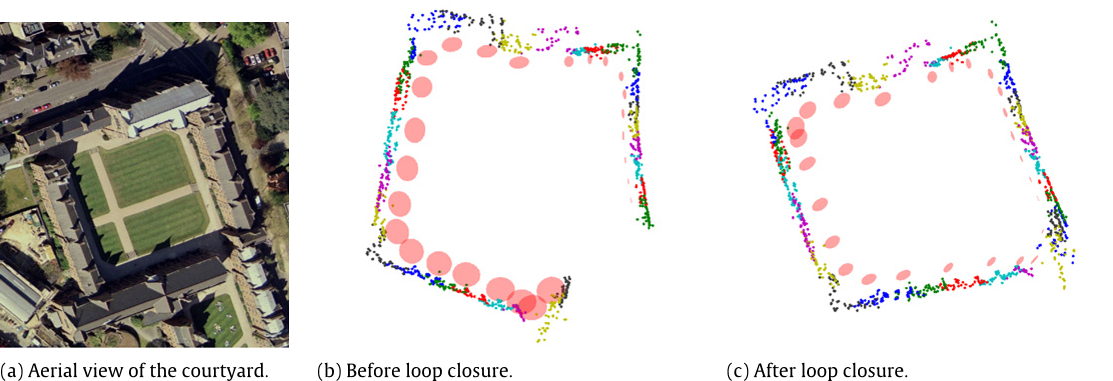
\includegraphics[width=0.8\textwidth]{imgs/loopClosure.png}
   \caption{Example of loop closure\label{fig:loopClose}}
\end{figure} 

In filter based SLAM, there is no easy way to implement this loop closure, particularly if previous locations have been saved in static submaps. In graph based SLAM, it is trivial to add an additional constraint between robot poses when a location is revisited, shown as function $f$ in Figure \ref{fig:loopClose2}. Optimising over this new graph automatically propogates error correction back through previous states.

\begin{figure}[H]
\centering
  % Graphic for TeX using PGF
% Title: /home/lach/uni/ursa/final_report/diagrams/loopclose.dia
% Creator: Dia v0.97.3
% CreationDate: Sun Oct 22 16:57:12 2017
% For: lach
% \usepackage{tikz}
% The following commands are not supported in PSTricks at present
% We define them conditionally, so when they are implemented,
% this pgf file will use them.
\ifx\du\undefined
  \newlength{\du}
\fi
\setlength{\du}{15\unitlength}
\begin{tikzpicture}
\pgftransformxscale{1.000000}
\pgftransformyscale{-1.000000}
\definecolor{dialinecolor}{rgb}{0.000000, 0.000000, 0.000000}
\pgfsetstrokecolor{dialinecolor}
\definecolor{dialinecolor}{rgb}{1.000000, 1.000000, 1.000000}
\pgfsetfillcolor{dialinecolor}
\definecolor{dialinecolor}{rgb}{1.000000, 1.000000, 1.000000}
\pgfsetfillcolor{dialinecolor}
\fill (16.000000\du,17.900000\du)--(16.000000\du,23.800000\du)--(33.000000\du,23.800000\du)--(33.000000\du,17.900000\du)--cycle;
\pgfsetlinewidth{0.100000\du}
\pgfsetdash{}{0pt}
\pgfsetdash{}{0pt}
\pgfsetmiterjoin
\definecolor{dialinecolor}{rgb}{0.000000, 0.000000, 0.000000}
\pgfsetstrokecolor{dialinecolor}
\draw (16.000000\du,17.900000\du)--(16.000000\du,23.800000\du)--(33.000000\du,23.800000\du)--(33.000000\du,17.900000\du)--cycle;
% setfont left to latex
\definecolor{dialinecolor}{rgb}{0.000000, 0.000000, 0.000000}
\pgfsetstrokecolor{dialinecolor}
\node at (24.500000\du,21.045000\du){};
\definecolor{dialinecolor}{rgb}{1.000000, 1.000000, 1.000000}
\pgfsetfillcolor{dialinecolor}
\pgfpathellipse{\pgfpoint{17.500000\du}{9.605834\du}}{\pgfpoint{1.500000\du}{0\du}}{\pgfpoint{0\du}{1.605834\du}}
\pgfusepath{fill}
\pgfsetlinewidth{0.100000\du}
\pgfsetdash{}{0pt}
\pgfsetdash{}{0pt}
\pgfsetmiterjoin
\definecolor{dialinecolor}{rgb}{0.000000, 0.000000, 0.000000}
\pgfsetstrokecolor{dialinecolor}
\pgfpathellipse{\pgfpoint{17.500000\du}{9.605834\du}}{\pgfpoint{1.500000\du}{0\du}}{\pgfpoint{0\du}{1.605834\du}}
\pgfusepath{stroke}
% setfont left to latex
\definecolor{dialinecolor}{rgb}{0.000000, 0.000000, 0.000000}
\pgfsetstrokecolor{dialinecolor}
\node at (17.500000\du,9.800834\du){r(0)};
\definecolor{dialinecolor}{rgb}{1.000000, 1.000000, 1.000000}
\pgfsetfillcolor{dialinecolor}
\pgfpathellipse{\pgfpoint{22.500000\du}{9.605834\du}}{\pgfpoint{1.500000\du}{0\du}}{\pgfpoint{0\du}{1.605834\du}}
\pgfusepath{fill}
\pgfsetlinewidth{0.100000\du}
\pgfsetdash{}{0pt}
\pgfsetdash{}{0pt}
\pgfsetmiterjoin
\definecolor{dialinecolor}{rgb}{0.000000, 0.000000, 0.000000}
\pgfsetstrokecolor{dialinecolor}
\pgfpathellipse{\pgfpoint{22.500000\du}{9.605834\du}}{\pgfpoint{1.500000\du}{0\du}}{\pgfpoint{0\du}{1.605834\du}}
\pgfusepath{stroke}
% setfont left to latex
\definecolor{dialinecolor}{rgb}{0.000000, 0.000000, 0.000000}
\pgfsetstrokecolor{dialinecolor}
\node at (22.500000\du,9.800834\du){r(1)};
\definecolor{dialinecolor}{rgb}{1.000000, 1.000000, 1.000000}
\pgfsetfillcolor{dialinecolor}
\pgfpathellipse{\pgfpoint{31.500000\du}{9.605834\du}}{\pgfpoint{1.500000\du}{0\du}}{\pgfpoint{0\du}{1.605834\du}}
\pgfusepath{fill}
\pgfsetlinewidth{0.100000\du}
\pgfsetdash{}{0pt}
\pgfsetdash{}{0pt}
\pgfsetmiterjoin
\definecolor{dialinecolor}{rgb}{0.000000, 0.000000, 0.000000}
\pgfsetstrokecolor{dialinecolor}
\pgfpathellipse{\pgfpoint{31.500000\du}{9.605834\du}}{\pgfpoint{1.500000\du}{0\du}}{\pgfpoint{0\du}{1.605834\du}}
\pgfusepath{stroke}
% setfont left to latex
\definecolor{dialinecolor}{rgb}{0.000000, 0.000000, 0.000000}
\pgfsetstrokecolor{dialinecolor}
\node at (31.500000\du,9.800834\du){r(T)};
\pgfsetlinewidth{0.100000\du}
\pgfsetdash{}{0pt}
\pgfsetdash{}{0pt}
\pgfsetbuttcap
{
\definecolor{dialinecolor}{rgb}{0.000000, 0.000000, 0.000000}
\pgfsetfillcolor{dialinecolor}
% was here!!!
\definecolor{dialinecolor}{rgb}{0.000000, 0.000000, 0.000000}
\pgfsetstrokecolor{dialinecolor}
\draw (19.000000\du,9.605830\du)--(21.000000\du,9.605830\du);
}
\pgfsetlinewidth{0.100000\du}
\pgfsetdash{}{0pt}
\pgfsetdash{}{0pt}
\pgfsetbuttcap
{
\definecolor{dialinecolor}{rgb}{0.000000, 0.000000, 0.000000}
\pgfsetfillcolor{dialinecolor}
% was here!!!
\definecolor{dialinecolor}{rgb}{0.000000, 0.000000, 0.000000}
\pgfsetstrokecolor{dialinecolor}
\draw (17.500000\du,17.900000\du)--(17.500000\du,11.211700\du);
}
\pgfsetlinewidth{0.100000\du}
\pgfsetdash{}{0pt}
\pgfsetdash{}{0pt}
\pgfsetbuttcap
{
\definecolor{dialinecolor}{rgb}{0.000000, 0.000000, 0.000000}
\pgfsetfillcolor{dialinecolor}
% was here!!!
\definecolor{dialinecolor}{rgb}{0.000000, 0.000000, 0.000000}
\pgfsetstrokecolor{dialinecolor}
\draw (22.500000\du,17.900000\du)--(22.500000\du,11.211700\du);
}
\pgfsetlinewidth{0.100000\du}
\pgfsetdash{}{0pt}
\pgfsetdash{}{0pt}
\pgfsetbuttcap
{
\definecolor{dialinecolor}{rgb}{0.000000, 0.000000, 0.000000}
\pgfsetfillcolor{dialinecolor}
% was here!!!
\definecolor{dialinecolor}{rgb}{0.000000, 0.000000, 0.000000}
\pgfsetstrokecolor{dialinecolor}
\draw (31.500000\du,17.900000\du)--(31.500000\du,11.211700\du);
}
% setfont left to latex
\definecolor{dialinecolor}{rgb}{0.000000, 0.000000, 0.000000}
\pgfsetstrokecolor{dialinecolor}
\node[anchor=west] at (17.900000\du,14.600000\du){g(0)};
% setfont left to latex
\definecolor{dialinecolor}{rgb}{0.000000, 0.000000, 0.000000}
\pgfsetstrokecolor{dialinecolor}
\node[anchor=west] at (18.885819\du,8.991308\du){u(0,1)};
% setfont left to latex
\definecolor{dialinecolor}{rgb}{0.000000, 0.000000, 0.000000}
\pgfsetstrokecolor{dialinecolor}
\node[anchor=west] at (22.900000\du,14.400000\du){g(1)};
% setfont left to latex
\definecolor{dialinecolor}{rgb}{0.000000, 0.000000, 0.000000}
\pgfsetstrokecolor{dialinecolor}
\node[anchor=west] at (32.250000\du,14.800000\du){g(T)};
\definecolor{dialinecolor}{rgb}{1.000000, 1.000000, 1.000000}
\pgfsetfillcolor{dialinecolor}
\pgfpathellipse{\pgfpoint{24.750000\du}{20.750000\du}}{\pgfpoint{1.750000\du}{0\du}}{\pgfpoint{0\du}{1.750000\du}}
\pgfusepath{fill}
\pgfsetlinewidth{0.100000\du}
\pgfsetdash{}{0pt}
\pgfsetdash{}{0pt}
\pgfsetmiterjoin
\definecolor{dialinecolor}{rgb}{0.000000, 0.000000, 0.000000}
\pgfsetstrokecolor{dialinecolor}
\pgfpathellipse{\pgfpoint{24.750000\du}{20.750000\du}}{\pgfpoint{1.750000\du}{0\du}}{\pgfpoint{0\du}{1.750000\du}}
\pgfusepath{stroke}
% setfont left to latex
\definecolor{dialinecolor}{rgb}{0.000000, 0.000000, 0.000000}
\pgfsetstrokecolor{dialinecolor}
\node at (24.750000\du,20.945000\du){m(x,y)};
\pgfsetlinewidth{0.100000\du}
\pgfsetdash{}{0pt}
\pgfsetdash{}{0pt}
\pgfsetbuttcap
{
\definecolor{dialinecolor}{rgb}{0.000000, 0.000000, 0.000000}
\pgfsetfillcolor{dialinecolor}
% was here!!!
\definecolor{dialinecolor}{rgb}{0.000000, 0.000000, 0.000000}
\pgfsetstrokecolor{dialinecolor}
\pgfpathmoveto{\pgfpoint{31.500183\du}{8.000085\du}}
\pgfpatharc{296}{245}{10.625000\du and 10.625000\du}
\pgfusepath{stroke}
}
% setfont left to latex
\definecolor{dialinecolor}{rgb}{0.000000, 0.000000, 0.000000}
\pgfsetstrokecolor{dialinecolor}
\node[anchor=west] at (27.000000\du,6.000000\du){f(1,T)};
% setfont left to latex
\definecolor{dialinecolor}{rgb}{0.000000, 0.000000, 0.000000}
\pgfsetstrokecolor{dialinecolor}
\node[anchor=west] at (27.500000\du,9.700000\du){...};
\pgfsetlinewidth{0.100000\du}
\pgfsetdash{}{0pt}
\pgfsetdash{}{0pt}
\pgfsetbuttcap
{
\definecolor{dialinecolor}{rgb}{0.000000, 0.000000, 0.000000}
\pgfsetfillcolor{dialinecolor}
% was here!!!
\definecolor{dialinecolor}{rgb}{0.000000, 0.000000, 0.000000}
\pgfsetstrokecolor{dialinecolor}
\draw (24.000000\du,9.605830\du)--(26.000000\du,9.600000\du);
}
% setfont left to latex
\definecolor{dialinecolor}{rgb}{0.000000, 0.000000, 0.000000}
\pgfsetstrokecolor{dialinecolor}
\node[anchor=west] at (23.885819\du,8.991308\du){u(1,2)};
\end{tikzpicture}

  \caption{Adding a new edge allows loop closure\label{fig:loopClose2}}
\end{figure}

The approach described above is very general, covers a wide variety of sensor configurations. For example, the authors in \cite{hong} and \cite{annaiyan} have applied this approach to visual sensors, while in \cite{vysotska} the authors used publically available mapping data to further describe the probability functions. \\

Graph based SLAM is a major area of research with significant complexities which have not been discussed in full detail above. A more comprehensive summary of the details of implementing graph based SLAM algorithms can be found at \cite{grisetti}. 

\section{Flight controllers}
In the majority of cases, researchers in UAV systems do not develop full flight control systems. However, many authors do conduct extensive tuning or system identification in order to improve the performance of commercial or open-source controllers. For example, in \cite{feicui} a comprehensive system identification process was undertaken, using the measured frequency response of four seperate input variables to a commercial controller: $\delta_\theta$, $\delta_x$, $\delta_y$, $\delta_z$. These variables induced responses in the yaw, pitch, roll and average motor speed respectively. Performance metrics were not provided after entering the identified system data into the controller.\\

In \cite{saengphet}, a detailed procedure is proposed to tune the PID parameters in the open source PX4 controller. The procedure consists of collecting data via piloted test flights, and using functions in \texttt{MATLAB} to tune the PID values. The authors claim some improvement in robustness over heuristic methods such as Ziegler-Nichols.\\

For more advanced flight patterns, more complex controllers are required. In particular, for a PID controller, an assumption of small values for roll and pitch is required. In \cite{wang}, the authors propose a neural network based method to remove this requirement, with a significant improvement in performance.\\

The major open source options for flight controllers are ArduPilot \footnote{\url{http://ardupilot.org/}} and PX4 \footnote{\url{http://px4.io/}}. Both systems utilise PID controllers.\\


\section{Navigation algorithms}


\end{document}

